
% DEFINE SOME HANDY SYMBOLS:
%\simlt and \simgt produce > and < signs with twiddle underneath
\def\spose#1{\hbox to 0pt{#1\hss}}
\def\simlt{\mathrel{\spose{\lower 3pt\hbox{$\mathchar"218$}}
     \raise 2.0pt\hbox{$\mathchar"13C$}}}
\def\simgt{\mathrel{\spose{\lower 3pt\hbox{$\mathchar"218$}}
     \raise 2.0pt\hbox{$\mathchar"13E$}}}
%\simpropto produces \propto with twiddle underneath
\def\simpropto{\mathrel{\spose{\lower 3pt\hbox{$\mathchar"218$}}
     \raise 2.0pt\hbox{$\propto$}}}
\def\tauc{\tau_\textrm{CMB}}

\newcommand{\acl}[1]{{\color{red} \textbf{[ACL:  #1]}}}

\documentclass[twocolumn,aps,prd,nofootinbib,showpacs]{revtex4-1}
\usepackage{amsmath,graphicx,bm,color}
\begin{document}
\title{Optical Depth from $21\,\textrm{cm}$}


\date{\today}



\pacs{95.75.-z,98.80.-k,95.75.Pq,98.80.Es}


\begin{abstract}

\end{abstract}

\maketitle

\section{Introduction}
\begin{itemize}
\item Reionization is not only an interesting epoch to study in its own right, but also because it's a nuisance for the CMB.  If we can understand reionization, we can predict $\tau_{CMB}$.  We can then send our prediction to our CMB friends so that they no longer have to marginalize over it.  In turn, that gives us better cosmological constraints on the other parameters.  This paper is timely because we have next-generation instruments (like HERA!) coming online.
\end{itemize}

\begin{equation}
\tau = \int  \sigma_T \langle x_e (z) n_\textrm{HI} (z) \rangle dl.
\end{equation}

\begin{equation}
\delta T_{b} \approx T_{b0} ( 1 - x_\textrm{HII} ) (1 + \delta)
\end{equation}

What are we going to do with the peculiar velocity term? (Also, I don't understand it).

\begin{equation}
\langle x_\textrm{HII} ( 1 + \delta) \rangle = \frac{\langle \delta T_b (z) \rangle - T_{b0}}{T_{b0}}
\end{equation}
\begin{equation}
\tau = \sigma_T (1 + f_\textrm{He}) \int dl \overline{n}_H (z) \frac{\langle \delta T_b (z) \rangle - T_{b0}}{T_{b0}}
\end{equation}

\section{Ingredients for a precise prediction of $\tau$ }

In practical terms, the optical depth $\tau$ is a nuisance parameter that is self-consistently fit for in CMB studies. While such an approach is attractive in that it does not require detailed models of reionization (or any other process that may produce free electrons), its downside is that one must simply accept any degeneracies in parameter fits. In particular, CMB experiments are much more sensitive to the overall combination of $A_s e^{-2\tau}$ than to $A_s$ or $\tau$ individually. To break such degeneracies, it is necessary to determine $\tau$ independently of the CMB data. Typically, this requires modeling the underlying astrophysics of reionization, and the goal in this section is to precisely describe the various quantities (both astrophysical and cosmological) that are needed for such modeling.

The optical depth is given by
\begin{equation}
\tau = \sigma_T \int    \overline{n}_e (z)  \frac{dl}{dz} dz,
\end{equation}
where $\sigma_T$ is the Thomson cross-section, $\overline{n}_e$ is the free-electron number density (with the overline denoting an average over all sky directions), and $dl/dz$ is the line-of-sight proper distance per unit redshift. Explicitly, $\overline{n}_e$ may be decomposed as
\begin{eqnarray}
\overline{n}_e &=& \overline{x_\textrm{HII} n_\textrm{H}} + \overline{x_\textrm{HeII} n_\textrm{He}} + \overline{x_\textrm{HeIII} n_\textrm{He}} \nonumber \\
&=& \overline{x_\textrm{HII} n_b} + \frac{1}{4}\overline{x_\textrm{HeIII} n_b}Y_p^\textrm{BBN} \nonumber \\
&=& \overline{n}_b \left[  \overline{x_\textrm{HII} (1+\delta_b)} + \frac{1}{4}\overline{x_\textrm{HeIII} (1+\delta_b)} Y_p^\textrm{BBN} \right],
\end{eqnarray}
where $n_\textrm{H}$, $n_\textrm{He}$, and $n_b = n_\textrm{H} + n_\textrm{He}$ are the hydrogen, helium, and baryon number densities, respectively. The ionization fractions (defined to be between $0$ and $1$) are given by $x_\textrm{HII}$, $x_\textrm{HeII}$, and $x_\textrm{HeIII}$, referring to singly ionized hydrogen, singly ionized helium, and doubly ionized helium, respectively. The helium fraction $Y_p^\textrm{BBN}$ is defined\footnote{We follow both the \emph{Planck} team's convention and notation in defining $Y_p^\textrm{BBN}$ as four times the number density fraction, rather than as the helium \emph{mass} fraction (defined as $4n_\textrm{He} / [n_\textrm{H} + (m_\textrm{He} / m_\textrm{H}) n_\textrm{H} ]$, where $m_\textrm{H}$ and $m_\textrm{He}$ are the atomic weights of hydrogen and helium, respectively).} as $4n_\textrm{He} / n_b$, and $\delta_b$ denotes the baryon overdensity. In the penultimate equality, we made the standard approximation that the helium is singly reionized at the same time as hydrogen is, and in the final equality, we used the fact that $n_b =\overline{n}_b ( 1+ \delta_b)$. With this factorization, the averaged baryon density can be easily related to cosmological parameters via
\begin{equation}
\overline{n}_b = \frac{3 H_0^2 \Omega_b}{8 \pi G \mu m_p} (1+z)^3,
\end{equation}
where $H_0$ is the Hubble parameter, $\Omega_b$ is the normalized baryon density, $G$ is the gravitational constant, $m_p$ is the mass of the proton, and $\mu$ is the mean molecular weight, which in our case is given by
\begin{equation}
\mu = 1 + \frac{Y_p^\textrm{BBN}}{4} \left( \frac{m_\textrm{He}}{m_\textrm{H}} - 1\right).
\end{equation}
Finally, we assume a flat universe and thus have as our differential line element
\begin{equation}
\frac{dl}{dz} =  \frac{c/H_0}{(1+z) \sqrt{\Omega_m (1+z)^3 + \Omega_\Lambda}}.
\end{equation}

Putting everything together, we may express the total optical depth as $\tau \equiv \tau_\textrm{H} + \tau_\textrm{He}$, with $\tau_\textrm{H}$ and $\tau_\textrm{He}$ denoting the portions of the optical depth sourced by free electrons from HI/HeI reionization and that from HeII reionization, respectively \acl{What's the latex command for changing the font for things like HI?}. These two contributions take the form
\begin{eqnarray}
\label{eq:tauH}
\tau_\textrm{H} = \frac{3 H_0 \Omega_b \sigma_Tc}{8 \pi G m_p} \left[ 1 + \frac{Y_p^\textrm{BBN}}{4}\left( \frac{m_\textrm{He}}{m_\textrm{H}} - 1\right)\right]^{-1} \nonumber \\
\times \int_0^{z_\textrm{CMB}} \frac{dz (1+z)^2}{\sqrt{\Omega_\Lambda + \Omega_m (1+z)^3}}  \overline{x_\textrm{HII} (1+\delta_b)},
\end{eqnarray} 
and
\begin{eqnarray}
\label{eq:tauHe}
\tau_\textrm{He} = \frac{3 H_0 \Omega_b \sigma_Tc}{8 \pi G m_p} \left[ \frac{4}{Y_p^\textrm{BBN}} + \left( \frac{m_\textrm{He}}{m_\textrm{H}} - 1\right)\right]^{-1} \nonumber \\
\times \int_0^{z_\textrm{CMB}} \frac{dz (1+z)^2}{\sqrt{\Omega_\Lambda + \Omega_m (1+z)^3}}  \overline{x_\textrm{HeIII} (1+\delta_b)},
\end{eqnarray}
where $z_\textrm{CMB}$ is the redshift of the surface of last scattering. From these expressions, we see explicitly how various cosmological parameters and astrophysical fields contribute to a prediction of $\tau$. In what follows, we will discuss the extent to which these contributions must be known accurately before a precision value for $\tau$ can be predicted.

\subsection{Uncertainties from fundamental constants and cosmological parameters}

Eqs. \eqref{eq:tauH} and \eqref{eq:tauHe} both involve a large number of fundamental constants and cosmological parameters, all of which come with their own error bars. Constants such as $G$, $\sigma_T$, $c$, $m_p$, $m_\textrm{H}$, and $m_\textrm{He}$ contribute negligibly to the error budget of $\tau$. The same is true for $Y_p^\textrm{BBN}$, which is constrained to be $0.2467\pm0.0006$ by a combination of \emph{Planck} data and Big Bang Nucleosynthesis (BBN) calculations \acl{Cite!}. The remaining parameters contribute to the error budget in a non-negligible way and must be accounted for.

Consider first the uncertainties arising from cosmological parameters, leaving astrophysical uncertainties in the reionization process to Sec. \ref{sec:astroUncertainties}. To simplify the latter in order to clarify the former, suppose (for this section only) that reionization occurs instantaneously at redshift $z_\textrm{ion}$ (with different values depending on whether one is discussing hydrogen or helium reionization, i.e., whether one is referring to Eqs. \ref{eq:tauH} or \ref{eq:tauHe}).\acl{Should write a footnote somewhere defining hydrogen and helium reionization once and for all} Terms such as $\overline{x_\textrm{HII} (1+\delta_b)}$ and $\overline{x_\textrm{HeIII} (1+\delta_b)}$ thus reduce to step functions that are $1$ for $z<z_\textrm{ion}$ and $0$ otherwise. The integrals in our expressions can then be evaluated analytically, yielding
\begin{eqnarray}
\label{eq:exactConstant}
\tau \propto \frac{h \Omega_b }{\Omega_m} \left[ \sqrt{\Omega_\Lambda + \Omega_m (1+z_\textrm{ion})^3} - 1 \right],
\end{eqnarray}
where we have employed the standard definition $H_0 \equiv 100h \frac{\textrm{km}/\textrm{s}}{\textrm{Mpc}}$, and have omitted the subscripts for $\tau_\textrm{HI}$ and $\tau_\textrm{He}$ in favor of a generic $\tau$ because the dependence on cosmological parameters are the same in either case.

To estimate the uncertainty in this prefactor for $\tau$, we propagate cosmological parameter uncertainties from \emph{Planck} results. To account for error correlations between different parameters, we use the publicly released covariance matrices to draw random samples of $\Omega_b h^2$, $\Omega_c h^2$, and $\theta_\textrm{MC}$, where $\Omega_c$ is the normalized cold dark matter density, and $\theta_\textrm{MC}$ is the CosmoMC software package's approximation to the angular size of the sound horizon at recombination. From this set, all the parameters necessary for evaluating Eq. \eqref{eq:exactConstant} can be obtained. Using \emph{Planck's} ``Planck TT + lowP" covariance from the 2015 data release (featuring relatively high $\Omega_m$ and $\tau$), the fractional error in Eq. \eqref{eq:exactConstant} is $1.40\%$. Similar results are obtained from the ``Planck TT,TE,EE + lowP + lensing + ext" (featuring relatively low $\Omega_m$ and $\tau$), with a fractional error of $0.75\%$. As we shall see later in this paper, this level of uncertainty is large enough to be non-negligible in a precision determination of $\tau$, but still small enough for the $21\,\textrm{cm}$-derived computation of $\tau$ in later sections to have a meaningful impact on bottom-line cosmological parameter errors.

\begin{figure*}[!]
	\centering
	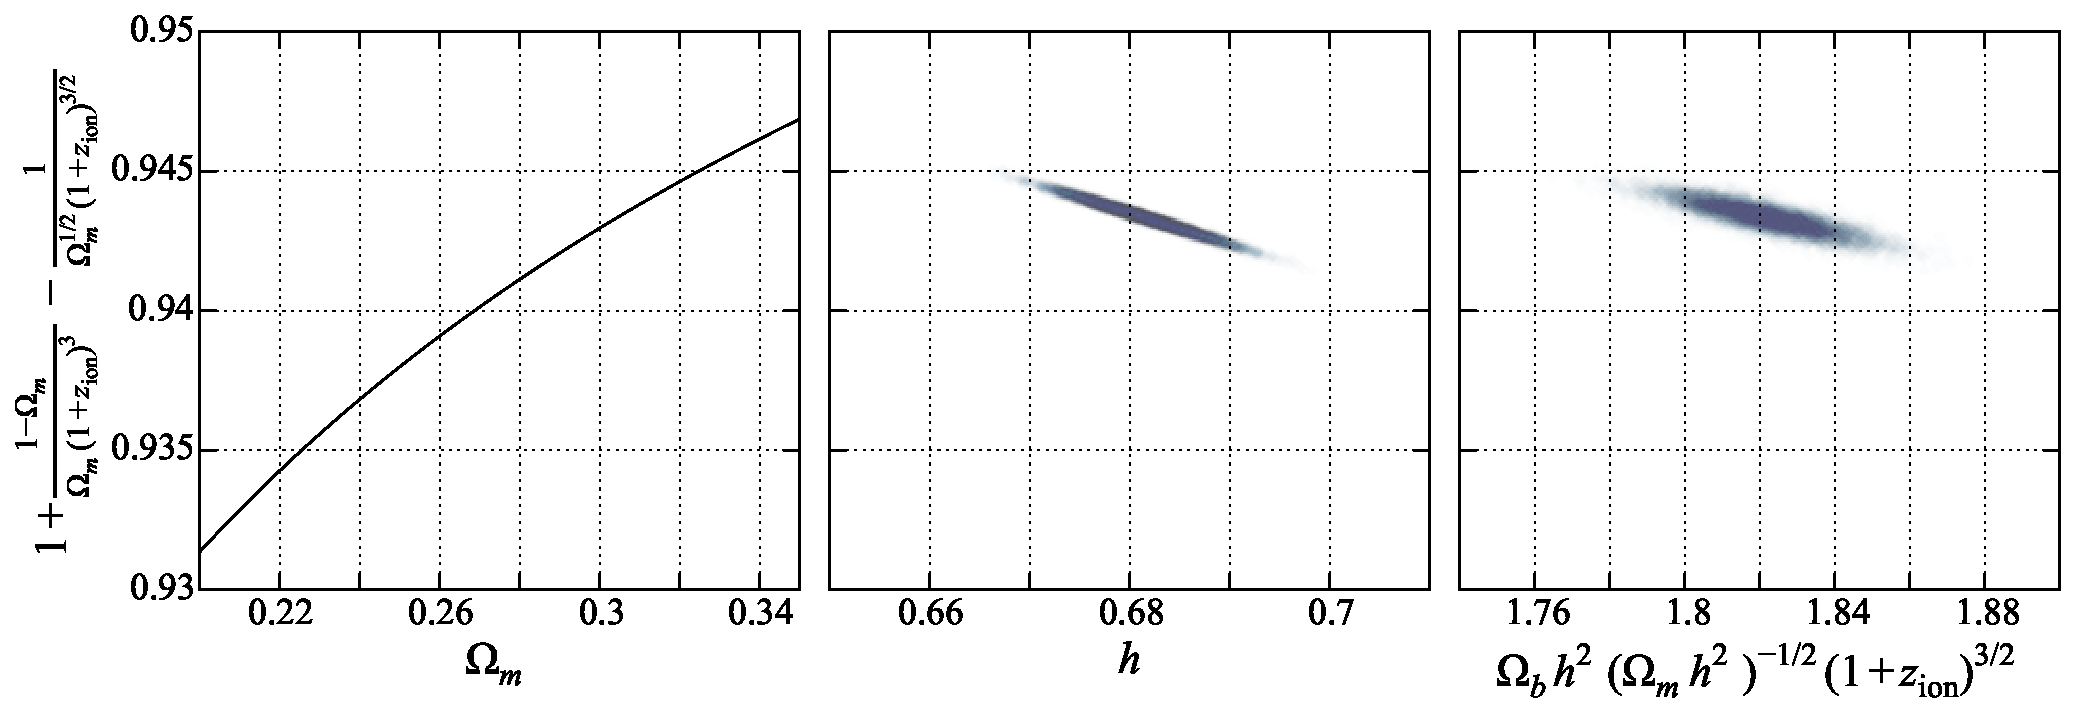
\includegraphics[width=1.0\textwidth,trim=0cm 0cm 0cm 0cm,clip]{figures/tauPrefac.pdf}
	\caption{asdf}
	\label{fig:tauPrefac}
\end{figure*}

Importantly, we note that the prefactor for $\tau$ is relatively insensitive to $h$. The fact that the error on our prefactor (about $0.75\%$ for Planck TT,TE,EE + lowP + lensing + ext) is roughly the same as the error on $h$ (about $0.46 / 67.74 \sim 0.68\%$ for the same dataset) is a coincidence, even though Eq. \eqref{eq:exactConstant} appears to be proportional to $h$. To understand this, assume that $\Omega_m (1+z)^3 \gg \Omega_\Lambda$. Taylor expanding our expression to first order then gives
\begin{equation}
\tau \propto \frac{\Omega_b h^2 (1+z_\textrm{ion})^\frac{3}{2}}{(\Omega_m h^2)^{1/2}} \left[ 1 + \frac{1-\Omega_m}{\Omega_m (1+z_\textrm{ion})^3}- \frac{1}{\Omega_m^{1/2} (1+z_\textrm{ion})^\frac{3}{2}}\right].
\end{equation}
where we have suggestively written the term in front of the brackets in terms of $(\Omega_m h^2,\Omega_b h^2)$. In this form, the parameters are proportional to physical energy densities, and are therefore directly related to our Universe's expansion history. CMB studies fit for  parameters like $\Omega_b h^2$ rather than $\Omega_b$. To zeroth order, then, the dependence on $h$ is cosmetic and cancels out completely, with $h$ entering only at first order with the appearance of a bare $\Omega_m$ inside the square brackets. Numerically, one finds that the term within the square brackets varies only slowly with $\Omega_m$, and thus any variations in $h$ are likely to have a small impact on our overall prefactor. This can be seen in Figure \ref{fig:tauPrefac}. The left panel shows samples of $\Omega_m$ plotted against samples of the first-order correction in the square brackets. One sees that a fractional change of order unity in $\Omega_m$ results in only a $2.5\%$ change in the first-order correction. The middle panel shows how the correction changes with $h$, with the former changing by $\sim 10\%$ for an order unity change in the latter. Finally, the right panel shows that the zeroth and first order corrections tend to have opposite signs, canceling out some of the uncertainty. Putting this all together, we see that our ability to constrain $\tau$ is reasonably insensitive to uncertainties in $h$. Indeed, we find from numerical experimentation that imposing a prior on $h$ has little to no effect on our ability to predict the $\tau$ prefactor. This is rather fortunate, for it shields us from the fact that \emph{Planck}-derived values of $h$ are in slight tension with direct $H(z)$ measurements using supernovae \acl{Cite!}. \acl{Need to mention the fact that since better constraints on $\tau$ give us better cosmological parameters all around, a joint fit will in principle push down the cosmological errors down even further. But it's negligible since $\Omega_b$ and $\Omega_m$ don't improve by that much.}



\subsection{Uncertainties from astrophysical processes}
\label{sec:astroUncertainties}

We now consider the astrophysical uncertainties in predicting $\tau$. At the crudest level, changes in astrophysics affect the redshift of reionization $z_\textrm{ion}$, which affects the optical depth via Eq. \eqref{eq:exactConstant}. Indeed, working in reverse and solving for $z_\textrm{ion}$ given a measured value of $\tau$ is how CMB experiments place constraints on reionization.

Ultimately, we shall see that it is important to model reionization astrophysics in detail, beyond the simple parametrization of $z_\textrm{ion}$. However, by considering the coarse dependence of $z_\textrm{ion}$ on $\tau$, we can distinguish the pieces of astrophysics that need to be carefully modeled from those that do not. In particular, we will now show that helium reionization contributes relatively little to $\tau$, making it unnecessary to model the process in a detailed way. Consider the ratio of $\tau_\textrm{He}$ to $\tau_\textrm{H}$, which can be written as
\begin{equation}
\frac{\tau_\textrm{He}}{\tau_\textrm{H}} = \frac{Y_p^\textrm{BBN}}{4} \left[ \frac{ \sqrt{\Omega_\Lambda + \Omega_m (1+z_\textrm{ion,He})^3} - 1}{ \sqrt{\Omega_\Lambda + \Omega_m (1+z_\textrm{ion,H})^3} - 1}\right],
\end{equation}
where $z_\textrm{ion,He}$ and $z_\textrm{ion,H}$ are the redshifts of helium and hydrogen reionization, respectively, assuming that both processes are instantaneous. For a fiducial model with $\Omega_\Lambda = 0.6911$, $\Omega_m = 0.3089$, $z_\textrm{ion,H} = 8.8$ (corresponding to \emph{Planck's} TT,TE,EE + lowP + lensing + ext dataset), and $z_\textrm{ion,He} = 3$, this ratio is $\sim 1.4\%$. Any errors in helium reionization are then suppressed by this factor. Quantitatively, if we parameterize the uncertainty in helium reionization by considering a shift $\delta z_\textrm{ion,He}$ in $z_\textrm{ion,He}$, the fractional error in $\tau$ arising from such uncertainty is given approximately by $\tau_\textrm{ion,H}^{-1} (\partial \tau_\textrm{He} / \partial z_\textrm{ion,He}) \delta z_\textrm{ion,He}$. This quantity is shown in Figure \ref{fig:HeII_reion_errors}, where we have overlaid the fractional errors from cosmological parameter uncertainties that we computed in the previous section. One sees that so long as the redshift of helium reionization $z_\textrm{ion,He}$ can be constrained to better than $ \delta z_\textrm{ion,He} \sim 1$, the uncertainties in the astrophysics of helium reionization are subdominant to the those from cosmological parameters.
%Assuming that the astrophysics of reionization is relatively insensitive to variations in cosmological parameters at the level of \emph{Planck} precision, the fractional errors from cosmological parameters and those from helium reionization combine in quadrature.
Current observational constraints suggest $ \delta z_\textrm{ion,He} \sim 0.1$ \acl{Cite Furlanetto \& Oh 2008 and see if there are better, more recent sources. Also need to mention how this is not precisely apples-to-apples, since we're converting a spatial spread in helium reionization to a spread in our knowledge.}, which make uncertainties from helium reionization negligible.

\begin{figure}[!]
	\centering
	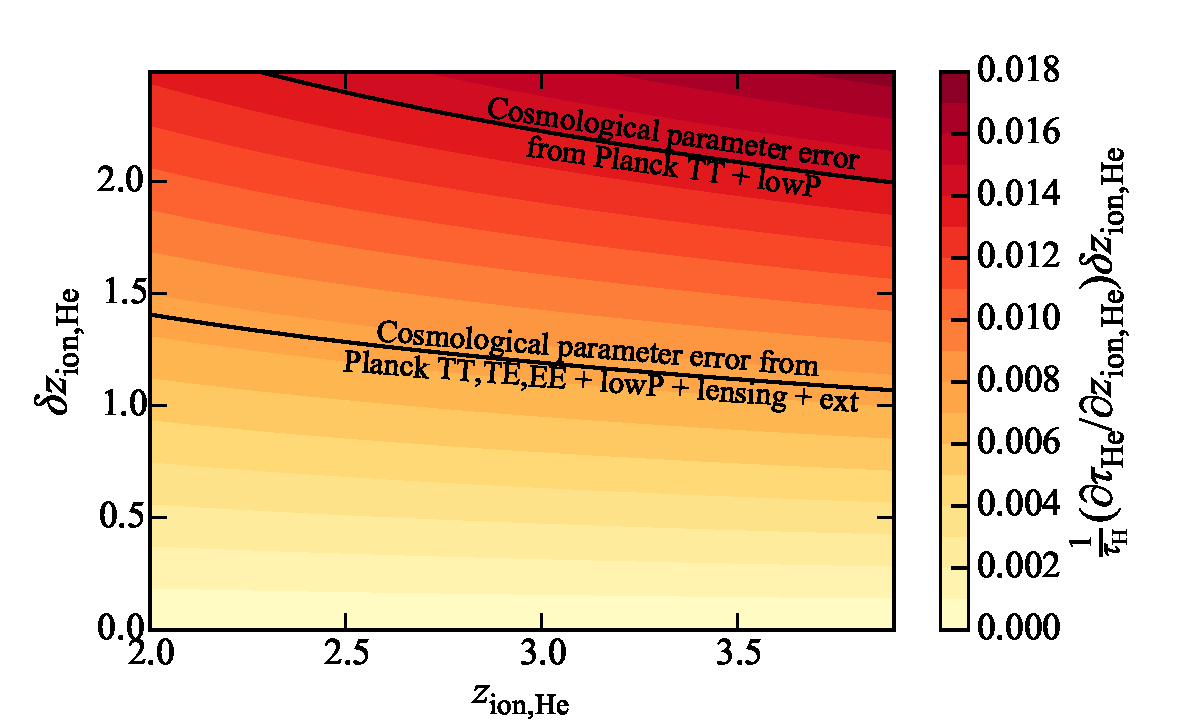
\includegraphics[width=0.5\textwidth,trim=0.5cm 0cm 0.75cm 0.90cm,clip]{figures/HeII_reion.pdf}
	\caption{asdf}
	\label{fig:HeII_reion_errors}
\end{figure}

In contrast, the astrophysics of hydrogen reionization must be accurately modeled for precise predictions of $\tau$. Repeating the above analysis for order unity perturbations in the $z_\textrm{ion,H}$, the resulting change in $\tau$ is $\sim 17\%$, largely because there is no longer a suppression by the ratio $\tau_\textrm{He} / \tau_\textrm{H}$. Of course, this is hardly surprising, for if changes in $z_\textrm{ion,H}$ did not generate reasonably large shifts in $\tau$, CMB-derived constraints on reionization would not exist. For our goal of predicting $\tau$ to be worthwhile, then, the details of hydrogen reionization must be understood. In fact, with hydrogen reionization dominating the CMB optical depth, one must also go beyond simple models of instantaneous reionization. To see this, consider the following numerical experiment. The astrophysics of reionization enters Eq. \eqref{eq:tauH} via the $\overline{x_\textrm{HII} (1+\delta_b)}$ term, the density-weighted ionized fraction. Crucially, it is incorrect to simplify this term to $\overline{x}_\textrm{HII}\overline{ (1+\delta_b)}$, since the $x_\textrm{HII}$ and $\delta_b$ may be spatially correlated, making the angular average of their product different from the product of their averages. In general, spatial correlations are an expected feature of reionization. For example, in ``inside-out" models of reionization, higher density regions produce a greater number of ionized photons and preferentially ionize first \acl{Cite some stuff}, resulting in a positive correlation between $x_\textrm{HII}$ and $\delta_b$. This is in contrast to ``outside-in" models, where the spectra of ionizing sources are typically harder, and the resulting ionizing radiation must redshift by a significant amount before being absorbed at far away, typically lower density regions. This results in a negative correlation. Figure \label{fig:InsideOutvsOutsideIn} shows the differential contributions to the total optical depth in various models \acl{Fill in more details}, all with the same mean ionization history $\overline{x}_\textrm{HII} (z) $. One sees that if the astrophysics of reionization is not properly accounted for, a $\sim 5$ to $10\%$ error is incurred in $\tau$.

\begin{figure}[!]
	\centering
	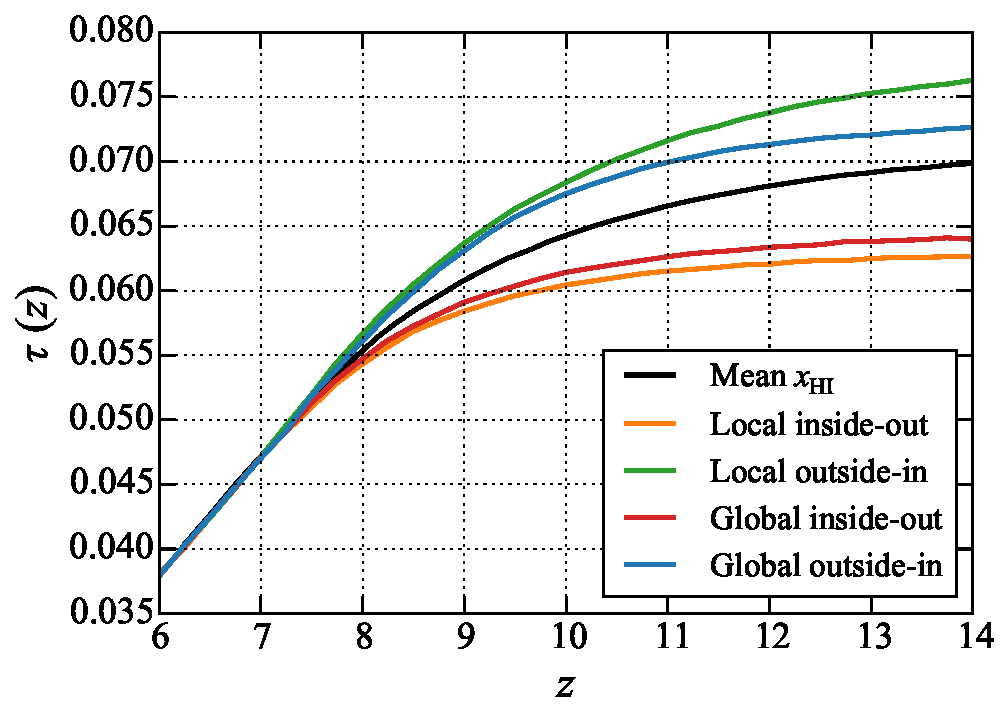
\includegraphics[width=0.5\textwidth,trim=0.5cm 0cm 0.5cm 0.80cm,clip]{figures/insideOutvsOutsideIn.pdf}
	\caption{asdf}
	\label{fig:InsideOutvsOutsideIn}
\end{figure}

In summary, we see that uncertainties in $\tau$ predictions arise from both uncertainties in cosmological parameters and uncertainties in astrophysics. If not accounted for in detail, the astrophysics contributes more to errors in $\tau$ than the cosmology does. To make progress, then, it is necessary to use external observational data to better understand reionization.

\section{Relating $\tau$ to HI surveys}

As a \emph{direct} probe of the IGM \acl{Make sure acronym is defined before this} at the relevant redshifts, it is unsurprising that one can use $21\,\textrm{cm}$ cosmological surveys to predict $\tau$. After all, $\tau$ and the $21\,\textrm{cm}$ line are both probes of reionization, and thus are sensitive to the same underlying astrophysics. In this section, however, we will argue that the connections between the $21\,\textrm{cm}$ line and $\tau$ are in fact much deeper, allowing the former to predict the latter much better than other probes of reionization can.

Consider first the expression for the CMB optical depth, which is given by
\begin{equation}
\tau = \int  \sigma_T \langle x_e (z) n_\textrm{HI} (z) \rangle dl,
\end{equation}
where $x_e$ is the free-electron fraction, $n_\textrm{HI}$ is the neutral hydrogen number density, $\sigma_T$ is the Thomson cross-section, $dl$ is the line-of-sight differential element \acl{Check to see if there's a better term for this}, and angle brackets $\langle \cdots \rangle$ denote an average over all sky directions. Importantly, this average does not factor, in the sense that $\langle x_e n_\textrm{HI} \rangle \neq \langle x_e  \rangle \langle n_\textrm{HI}  \rangle$, even though this approximation is frequently seen in the literature. Physically, this arises because there is a non-zero correlation between the ionization field (which governs the distribution of free electrons) and the density field during reionization. For example, in ``inside-out" reionization models, high density regions are ionized first, leading to a positive correlation between the ionization and density fields. Modeling such correlations are crucial to precision predictions of $\tau$.

Fortunately, the $21\,\textrm{cm}$ line can be an incisive probe of the relevant correlations. To see this, note that if one ignores peculiar velocities 

\section{Tau Predictions}

\begin{itemize}
\item What does it take to predict tau? Emphasize the point that Jonathan made: it's the density-weighted ionization fraction that counts. So it's more complicated than just integrating an ionization history. Perhaps this would be a good place to add Jonathan's nice plots from global inside-out, outside-in, local... etc.?
\end{itemize}

Roughly speaking, we envision a multi-stage process for using $21\,\textrm{cm}$ measurements for constraining $\tauc$. First, qualitatively different models are distinguished from one another with coarse measurements of the power spectrum or even higher order statistics \acl{Cite Watkinson and Pritchard}. Having selected a single model out of many, one then uses precision power spectrum measurements to fix free parameters within the model. The correlated ionization and density fields of the model can then be predicted from simulations, and the optical depth estimated. This simulation-derived optical depth may, however, deviate from the ``true" value of $\tauc$ in our Universe because simulations depend on random realizations of density fields. If this ``simulation variance" on $\tauc$ is small enough to be tolerable, one may immediately feed the derived value of $\tauc$ into broader cosmological parameter estimations. On the other hand, if the simulation variance is large, it becomes necessary to directly measure the realization of $\tauc$ that represents our Universe. To do so, we propose using power spectrum measurements to restrict the space of possible reionization histories, enabling a principal component-based parameterization that can then be precisely constrained using a global signal measurement. Through the linearity arguments presented above \acl{Make sure these are included, or discuss them here}, these essentially constitute a direct measurement of the optical depth.

\subsection{Tau predictions from power spectrum measurements}
\begin{itemize}
\item Power spectrum measurements are a rather poor way of doing it, but they're the most promising short-term observable. So we're choosing to take a look at it, even though it's quite model dependent. It'll essentially require tying the measurements to simulations. We assume that large qualitative changes to reionization physics have already been ruled out in an earlier model selection step.
\item Talk about the models and why it's ok to ignore spin temperature (basically ionization frac is too low when spin temperature effects are important). But maybe we should quantify this a little.
\item Point out the interesting feature where the degeneracies in 21cm don't compromise our ability to predict tau.

Of course, no probe of reionization is perfect, and any practical measurement will come with its attendant errors and degeneracies. For example, in \acl{Cite Jonnie and Grieg \& Mesinger} it was shown that except in the extremely high signal-to-noise regime, fits to theoretical model parameters from $21\,\textrm{cm}$ power spectrum measurements are prone to strong degeneracies if performed at a single redshift. Multi-redshift observations break these degeneracies to a great extent, enabling for instance $\sim 10\%$ level constraints \acl{Check numbers} from upcoming instruments like HERA. However, some degeneracy will remain, as evidenced by the elliptical contours shown in Figure \ref{fig:21cmDegen_wTau}, which show some example $68\%$ and $95\%$ confidence regions on $T_\textrm{vir}$ and $\zeta$ constraints. These are derived from Fisher matrix forecasts assuming multi-redshift power spectrum measurements performed by HERA \acl{Specify a lot more what went into this calculation, especially regarding foregrounds}. There is clearly a degeneracy that persists between the two parameter.

\begin{figure}[!]
	\centering
	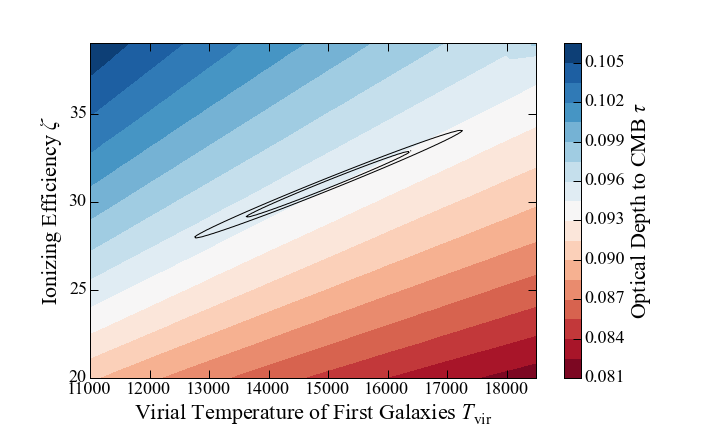
\includegraphics[width=0.5\textwidth]{figures/21cmDegen_wTau.png}
	\caption{asdf}
	\label{fig:21cmDegen_wTau}
\end{figure}

Fortunately, these residual degeneracies have relatively impact on one's ability to predict $\tau$. Performing a simulation of the ionization field for every point in the parameter space shown in Figure \label{fig:21cmDegen_wTau}, the relevant integral \acl{Reference the equation} can be evaluated to give predictions for $\tau$. The resulting solid color contours in Figure \label{fig:21cmDegen_wTau} are seen to be quite closely aligned to elliptical contours, suggesting that a very precise value for $\tau$ can be obtained from $21\,\textrm{cm}$ measurements even in the face of degeneracies.

\item Show $\tau$ predictions for both a WMAP-style redshift and a (probably lower tau) Planck redshift.
\item Talk about whether a bigger array does much better.
\end{itemize}
\subsection{Tau predictions from global signal measurements}
\begin{itemize}
\item Show that global signal measurements can get to precisely the quantity we need. But we need to limit the number of degrees of freedom in our fits in order for it to work.
\item Power spectrum measurements can help to provide a basis for global signal measurements. Show PCA modes for deviations from fiducial signal.

\begin{figure}[!]
	\centering
	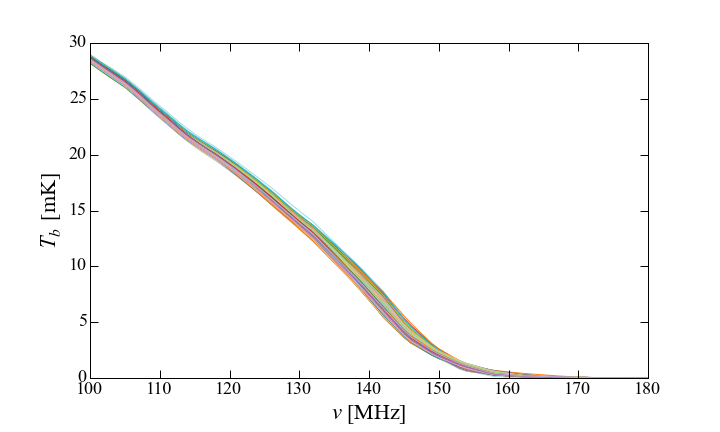
\includegraphics[width=0.5\textwidth]{figures/sampled_Tb_cutoff.png}
	\caption{asdf}
	\label{fig:sampled_Tb_cutoff}
\end{figure}

\begin{figure}[!]
	\centering
	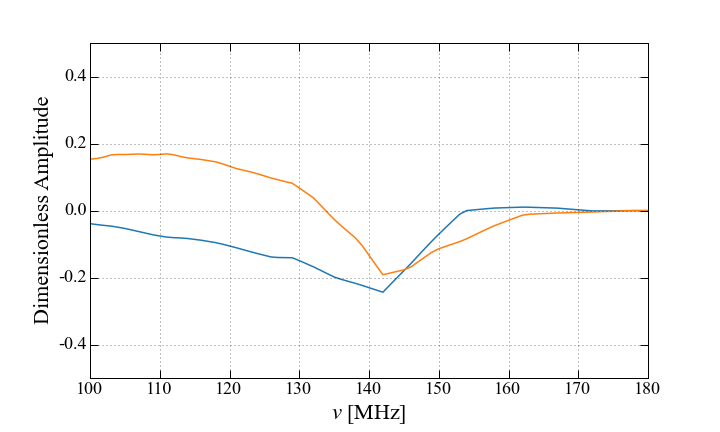
\includegraphics[width=0.5\textwidth]{figures/PCA_cutoff.png}
	\caption{asdf}
	\label{fig:PCA_cutoff}
\end{figure}


\begin{figure}[!]
	\centering
	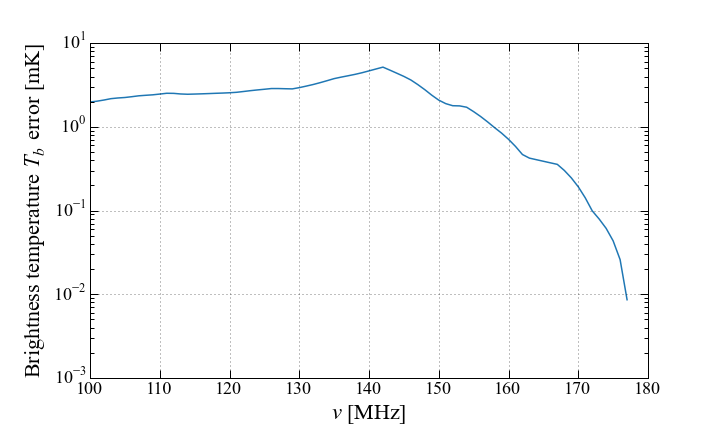
\includegraphics[width=0.5\textwidth]{figures/Tb_global_errors.png}
	\caption{asdf}
	\label{fig:Tb_global_errors}
\end{figure}

\item Some forecasts for constraining these deviation modes. Show different foreground subtraction scenarios.
\item Point out the fact that by making a direct measurement, we avoid the problem of cosmic variance, since we're essentially measuring ``our" tau, in our branch of the multiverse.
\end{itemize}
%\subsection{Tau predictions from imaging experiments}
%\item As far as predicting tau is concerned, an imaging experiment is just a very high signal-to-noise global signal experiment.
%\item However, one must be careful because an interferometer does not measure the zero-mode spatially. Need to rely on the assumption that at the relevant redshifts, we are in emission, so the brightness temperature is greater than or equal to zero. This lets us recover the zero-point.
%\item Perform thermal noise calculation.
%\item Give tau predictions
%\end{itemize}
\subsection{Summary of tau predictions}
\begin{itemize}
\item Provide a table summarizing values.
\end{itemize}

\section{Improvements in the CMB}
\subsection{Degeneracy breaking}
Highlight some specific examples.
\begin{itemize}
\item How might it be helpful to no longer have the $A_s$ and $\tau$ degeneracy? Translate the constraints into $\sigma_8$. This is interesting because it'll make it so that the cluster vs. CMB cosmological parameter tension either goes away or becomes statistically significant.

\begin{figure}[!]
	\centering
	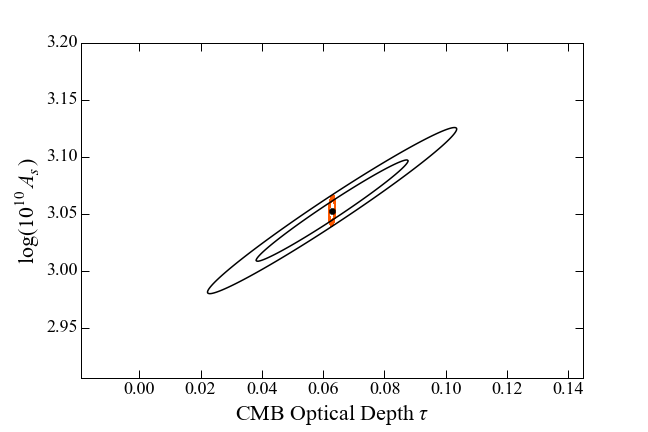
\includegraphics[width=0.5\textwidth]{figures/AsTau_w21cm.png}
	\caption{asdf}
	\label{fig:AsTau_w21cm}
\end{figure}

\item What about B-modes? Reionization bump predictions need $\tau$, so consistency tests are helped by 21cm. Also discuss Mortonson \& Hu (2008) and how inflationary parameters are biased if reionization not modeled correctly.
\acl{Ok, it turns out that the main degeneracy is between $r$ and $n_t$. It's true that $\tau$ is also degenerate with these parameters, but the degeneracy is sub-dominant compared to the one between $n_t$ and $r$. So improving $\tau$ does not really improve the bottom line for consistency-relation tests, since our knowledge of $\tau$ isn't the limiting factor.}
\end{itemize}

\section{Predictions for $x_{HI}$}
Mention how even thought it's not $x_{HI}$ that's directly relevant for $\tau$, the same measurements mentioned earlier might provide a way to probe the ionized fraction (particularly the power spectrum measurements).
\begin{itemize}
\item Show some projections for $x_{HI}$.
\item Talk about how this can be very complementary to optical/IR measurements.
\end{itemize}

\section{Conclusions}
Summarize our main points.

\section*{Acknowledgments}


\bibliography{21cmTau}


\end{document}
